\section{Test Plan}
In order to verify the correctness of the system the following tests were made:
\begin{enumerate}
	\item \textbf{Unit Tests}: following the \textbf{bottom-up} strategy, each sub-module (Parallel Multiplier, Ripple Carry Adder Pipelined...), after completing the implementation, has a dedicated testbench in order to check the correctness of the single sub-module in isolation. Considering the fact that this test are \textbf{trivial} (just checking if the sum or the product of some numbers is correct) this will not be showed in this documentation.
	\item \textbf{System Estimation Test}: in this phase, some testbenches were written with particular inputs. The aim of this test is only to check if the result will resemble the sigmoid curve by varying the inputs in time in an increasing way.
	\item \textbf{System Aimed Test}: after checking that the system is \textit{likely} correct by the latter test, through a python script will be made a test with different inputs in the range considered and check, with an additional testbench, if the outputs are equal.
\end{enumerate}
\subsection{System Estimation Test}
Even before checking the correctness of the output of the system by a given input, three "estimation tests" were made. The aim of these tests is just to obtain a sigmoid curve by setting each $x_{i}$ and $w_{i}$ and varying the bias $b$ in the range of $[-1; +1]$.
\subsubsection{Estimation Test 1}
In this case we have the following inputs:
\begin{equation}
	x_{1} \dots x_{10} = 0, w_{1} \dots w_{10} = 0
\end{equation}
The bias b will vary in the whole range of $[-1, +1]$. Just to remind the sigmoid function curve, we expect to obtain a curve with an odd symmetry and a "linear" behaviour, due to the fact that we are considering the values near zero of the curve:
\begin{figure}[H]
	\centering
	\caption{Sigmoid Function Plot}
	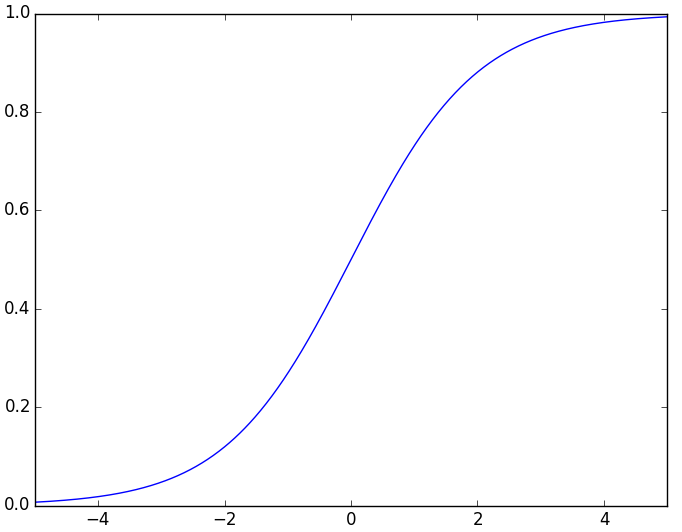
\includegraphics[width=8cm]{img/sigmoid.png}
\end{figure}
The output of the system is the following:
\begin{figure}[H]
	\centering
	\caption{Output of the System 1}
	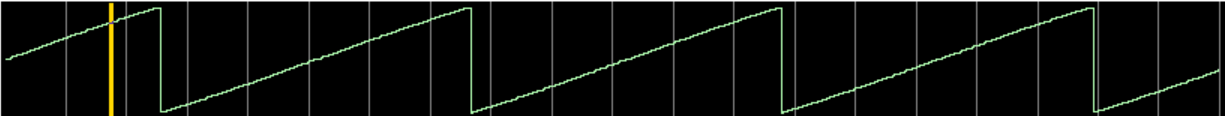
\includegraphics[width=\textwidth]{img/est_test_1.png}
\end{figure}
There are different replication of the system due to the fact that the bias b will "turn back" when he will get to his maximum. We can state that, by comparing the two figures, the \textbf{first estimation test is passed}. 
\subsubsection{Estimation Test 2}
\begin{equation}
	x_{1} \dots x_{10} \approx 1, w_{1} \dots w_{10} \approx 1
\end{equation}
The bias b will vary in the whole range of $[-1, +1]$. We expect to obtain a likely flat curve with some "high values" due to the fact that the summation of the ten product is 10 and the sigmoid at that value tends to 1.
\begin{figure}[H]
	\centering
	\caption{Output of the System 2}
	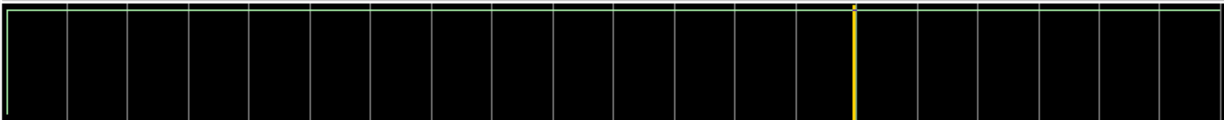
\includegraphics[width=\textwidth]{img/est_test_2.png}
\end{figure}
The output of the system is similar to a flat curve. We can state that, by comparing the system output with what we expected, the \textbf{second estimation test is passed}.
\subsubsection{Estimation Test 3}
\begin{equation}
	x_{1} \dots x_{10} \approx -1, w_{1} \dots w_{10} \approx 1
\end{equation}
The bias b will vary in the whole range of $[-1, +1]$. We expect to obtain a likely flat curve with some "low values" due to the fact that the summation of the ten product is -10.
\begin{figure}[H]
	\centering
	\caption{Output of the System 3}
	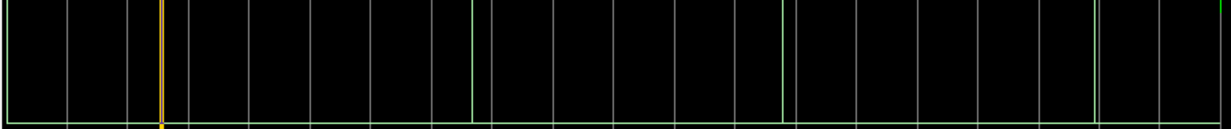
\includegraphics[width=\textwidth]{img/est_test_3.png}
\end{figure}
The curve is flat with low values but we can notice some \textit{noise}. This is due to the fact that to obtain a proper output some clock cycles are needed: this will lead to obtain intermediate results that are not good. But we can state that, by comparing the system output with what we expected, the \textbf{third estimation test is passed}.
\subsection{System Aimed Test}
At this point will be carried out some tests with the same inputs using the \textbf{Perceptron} architecture realized at this point and a \textit{python script} which will simulate the desired behaviour of the \textbf{Perceptron}. The latter is described through the following script:

\begin{lstlisting}[language=python]
import math

def get_outputs(i, x, w, b):
	print(f"################### TEST #{i} ###################")
	print(f"X: {x}")
	print(f"W: {w}")
	print(f"b: {b}")
	
	sum = summation(x, w, b)
	print(f"Sum result:\t\t\t\t {sum}")
	
	f_z = sigmoid_output(sum)
	print(f"Sigmoid output:\t\t\t {f_z}")
	
	#the sum with 12 bits
	sum_in_circuit = round(sum/lsb_in)
print(f"Sum value quantized:\t {sum_in_circuit}")

f_z_in_circuit = round(f_z/lsb_out)
	print(f"Output value quantized:\t {f_z_in_circuit}")
	def summation(x, w, b):
	sum = 0
	for i in range(0, 10):
	sum += x[i]*w[i]
	sum += b
	return sum

def sigmoid_output(s):
	res = (1)/(1 + math.exp(-s))
	return res

lsb_out = (1)/(2**15 - 1)
lsb_in = (32)/(2**11 - 1)
#Test #1
x = [-1,-1,-1,-1,-1,-1,-1,-1,-1,-1]
w = [1,1,1,1,1,1,1,1,1,1]
b = 0
get_outputs(1, x, w, b)
...
#Other tests
...
\end{lstlisting}

By running the python script the following output has been displayed in the console:

\begin{lstlisting}
################### TEST #1 ###################
X: [-1, -1, -1, -1, -1, -1, -1, -1, -1, -1]
W: [1, 1, 1, 1, 1, 1, 1, 1, 1, 1]
b: 0
Sum result:				 -10
Sigmoid output:			 4.5397868702434395e-05
Sum value quantized:	 -640
Output value quantized:	 1
################### TEST #2 ###################
X: [-0.75, -0.75, -0.75, -0.75, -0.75, -0.75, -0.75, -0.75, -0.75, -0.75]
W: [1, 1, 1, 1, 1, 1, 1, 1, 1, 1]
b: 0
Sum result:				 -7.5
Sigmoid output:			 0.0005527786369235996
Sum value quantized:	 -480
Output value quantized:	 18
################### TEST #3 ###################
X: [-0.5, -0.5, -0.5, -0.5, -0.5, -0.5, -0.5, -0.5, -0.5, -0.5]
W: [1, 1, 1, 1, 1, 1, 1, 1, 1, 1]
b: 0
Sum result:				 -5.0
Sigmoid output:			 0.0066928509242848554
Sum value quantized:	 -320
Output value quantized:	 219
################### TEST #4 ###################
X: [-0.5, -0.5, -0.5, -0.5, -0.5, -0.5, -0.5, -0.5, -0.5, -0.5]
W: [0.5, 0.5, 0.5, 0.5, 0.5, 0.5, 0.5, 0.5, 0.5, 0.5]
b: 0
Sum result:				 -2.5
Sigmoid output:			 0.07585818002124355
Sum value quantized:	 -160
Output value quantized:	 2486
################### TEST #5 ###################
X: [-0.5, -0.5, -0.5, -0.5, -0.5, -0.5, -0.5, -0.5, -0.5, -0.5]
W: [0, 0, 0, 0, 0, 0, 0, 0, 0, 0]
b: 0
Sum result:				 0.0
Sigmoid output:			 0.5
Sum value quantized:	 0
Output value quantized:	 16384
################### TEST #6 ###################
X: [-0.5, -0.5, -0.5, -0.5, -0.5, -0.5, -0.5, -0.5, -0.5, -0.5]
W: [-0.5, -0.5, -0.5, -0.5, -0.5, -0.5, -0.5, -0.5, -0.5, -0.5]
b: 0
Sum result:				 2.5
Sigmoid output:			 0.9241418199787566
Sum value quantized:	 160
Output value quantized:	 30281
################### TEST #7 ###################
X: [0.5, 0.5, 0.5, 0.5, 0.5, 0.5, 0.5, 0.5, 0.5, 0.5]
W: [1, 1, 1, 1, 1, 1, 1, 1, 1, 1]
b: 0
Sum result:				 5.0
Sigmoid output:			 0.9933071490757153
Sum value quantized:	 320
Output value quantized:	 32548
################### TEST #8 ###################
X: [0.75, 0.75, 0.75, 0.75, 0.75, 0.75, 0.75, 0.75, 0.75, 0.75]
W: [1, 1, 1, 1, 1, 1, 1, 1, 1, 1]
b: 0
Sum result:				 7.5
Sigmoid output:			 0.9994472213630764
Sum value quantized:	 480
Output value quantized:	 32749
################### TEST #9 ###################
X: [1, 1, 1, 1, 1, 1, 1, 1, 1, 1]
W: [1, 1, 1, 1, 1, 1, 1, 1, 1, 1]
b: 0
Sum result:				 10
Sigmoid output:			 0.9999546021312976
Sum value quantized:	 640
Output value quantized:	 32766
################### TEST #10 ###################
X: [1, 1, 1, 1, 1, 1, 1, 1, 1, 1]
W: [1, 1, 1, 1, 1, 1, 1, 1, 1, 1]
b: 1
Sum result:				 11
Sigmoid output:			 0.999983298578152
Sum value quantized:	 704
Output value quantized:	 32766
################### TEST #11 ###################
X: [-1, -1, -1, -1, -1, -1, -1, -1, -1, -1]
W: [1, 1, 1, 1, 1, 1, 1, 1, 1, 1]
b: -1
Sum result:				 -11
Sigmoid output:			 1.670142184809518e-05
Sum value quantized:	 -704
Output value quantized:	 1
\end{lstlisting}

By running a new testbench with \textbf{likely} the same inputs the following results were displayed in \textbf{Modelsim}:
\begin{figure}[H]
	\centering
	\caption{Output of the System 3}
	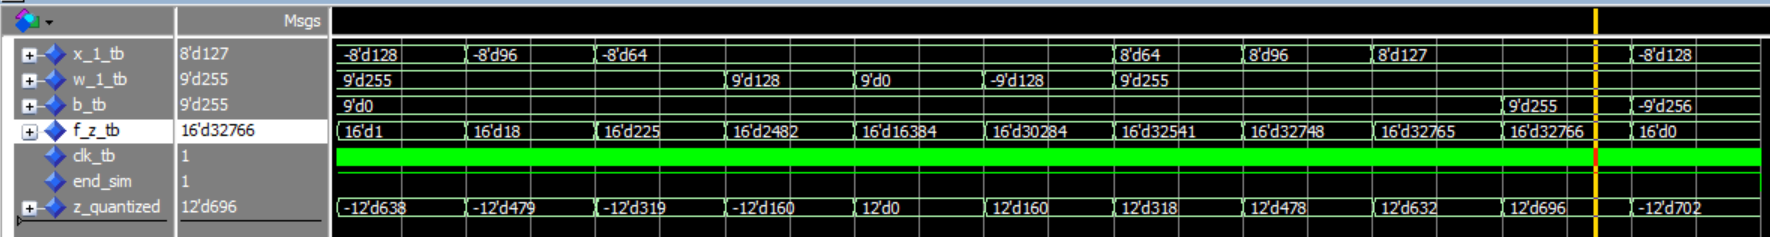
\includegraphics[width=\textwidth]{img/aimed_test.png}
\end{figure}

A comparison with the outputs can be seen in the following table:
\begingroup
\setlength{\tabcolsep}{10pt} % Default value: 6pt
\renewcommand{\arraystretch}{2} % Default
\begin{center}
	\begin{tabular}{|p{2cm}||p{2.4cm}|p{2.4cm}|p{2.4cm}|p{2.4cm}|}
		\hline
		\multirow{2}{*}{\textbf{Test}}  & \multicolumn{2}{|p{3cm}|}{\textbf{Python Script}} & \multicolumn{2}{|p{3cm}|}{\textbf{Modelsim}} \\
		\cline{2-5}
		 & $round\left(\dfrac{z}{LSB}\right)$ & $round\left(\dfrac{f(z)}{LSB}\right)$ &  $round\left(\dfrac{z}{LSB}\right)$ & $round\left(\dfrac{f(z)}{LSB}\right)$ \\
		\hline
		Test $\#$1 & -640 & 1 & -638 (+2) & 1 (=)\\
		Test $\#$2 & -480 & 18 & -479 (+1) & 18 (=)\\
		Test $\#$3 & -320 & 219 & -319 (+1) & 225 (+5)\\
		Test $\#$4 & -160 & 2486 & -160 (=) & 2482 (-4)\\
		Test $\#$5 & 0 & 16384 & 0 (=) & 16384 (=)\\
		Test $\#$6 & 160 & 30281 & 160 (=) & 30284 (+3)\\
		Test $\#$7 & 320 & 32548 & 318 (-2) & 32541 (-7)\\
		Test $\#$8 & 480 & 32749 & 478 (-2) & 32748 (-1)\\
		Test $\#$9 & 640 & 32766 & 632 (-8) & 32765 (-1)\\
		Test $\#$10 & 704 & 32766 & 696 (-8) & 32766 (=)\\
		Test $\#$11 & -704 & 1 & -702 (+2) & 0 (-1)\\
		\hline
	\end{tabular}
\end{center}
\endgroup

In the latter table are compared the z and f(z) (See Equation (1) and (2) for further details) as they are represented in the architecture: with a C2 representation.\\ 
As we can see in the latter table the outputs are \textbf{likely} the same, with some few differences that can be ignored. These differences can be easily explained: \textbf{Python's float} number will use \textbf{64 bits} instead of 12 or 16 as in our case. This difference will change the outputs, in fact, in our case, the number $+1$ ("01111111" in base of $x_{i}$ with 8 bits), for example, can't be represented precisely with a finite number of bits: so, the higher number of bits are available, the higher precision will be granted. All things considered, we can state \textbf{the system has passed the System Aimed Test} and, for our purpose, \textbf{can be considered verified.}